\chapter{Result}
Appendix \ref{appendix:raw} contains other results in raw data from the conducted evaluation.


\section{Performance Overhead}
The results from benchmarking the application on DaCapo Benchmark Suit \parencite{dacapo} is seen in Figure \ref{fig:Time} and \ref{fig:Memory}. Both graphs are constructed to show the added overhead of running the applications with Dynamic Taint Tracking activated. The graphs are conducted based on the data in Table \ref{TimeTable} and \ref{MemoryTable}.


\subsection{Time}
Figure \ref{fig:Time} displays the results of the average time overhead per application. The results show that the application with the least average time overhead was Tradesoap where 14.7\% was added. The largest application however, was Fop with an additional of 426.2\%. The average overall overhead is 142.1\%.

From the Tables \ref{TimeTable} can we as well see that the variation between the minimum and maximum time will for all applications be 437.8\%.

\begin{figure}[!h]
	\centering
	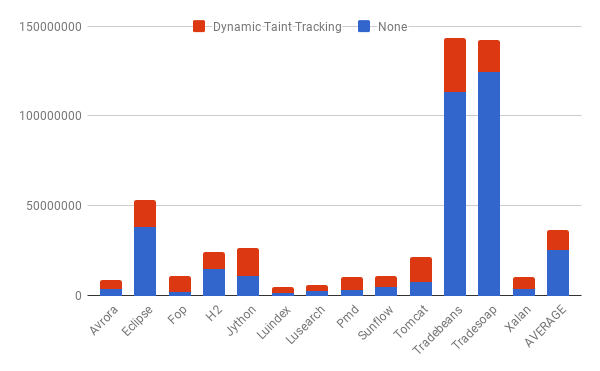
\includegraphics[width=\textwidth]{images/Time.png}
	\caption{Average Added Time in Microseconds}
	\label{fig:Time}
\end{figure}


\subsection{Memory}
Figure \ref{fig:Memory} displays the results of the average memory overhead per application. The results show that the application with the least average memory overhead was Eclipse where 5.5\% was added. The largest application however, was Fop with an additional of 277.8\%. The average overall overhead is 127.2\%.

From the Table \ref{MemoryTable} can we as well see that the variation between the minimum and maximum memory will for all 3.05.3\%.

\begin{figure}[!h]
	\centering
	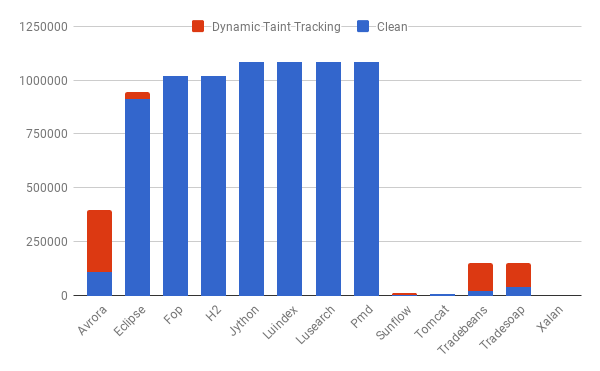
\includegraphics[width=\textwidth]{images/Memory.png}
	\caption{Average Added Memory in Kilobytes}
	\label{fig:Memory}
\end{figure}



\section{Applications}
ADD TABLE CAPTION DESCRIPTIONS!!!!



\begin{table}[!h]
  \centering
  \caption{Stanford SecuriBench Micro}
  \label{table:MicroTable}
  \resizebox{\columnwidth}{!}{
    \begin{tabular}{rcc}
                                                                & \textbf{Clean} & \textbf{Dynamic Taint Tracking} \\
      \textbf{SQL Injection (High (Medium))}                    & 20             & 0                               \\
      \textbf{Cross Site Scripting (Reflected) (High (Medium))} & 2              & 0                               \\
      \textbf{Cross Site Scripting (Reflected) (High (Low))}    & 69             & 0                               \\
      \textbf{Web Browser XSS Protection Not Enabled}           & 1              & 0                              
    \end{tabular}
  }
\end{table}


\begin{table}[!h]
  \centering
  \caption{Insecure}
  \label{table:InsecureTable}
  \resizebox{\columnwidth}{!}{
    \begin{tabular}{rcc}
                                                                & \textbf{Clean} & \textbf{Dynamic Taint Tracking} \\
      \textbf{SQL Injection (High (Medium))}                    & 4              & 0                               \\
      \textbf{Cross Site Scripting (Reflected) (High (Medium))} & 2              & 0                              
    \end{tabular}
  }  
\end{table}

\begin{table}[!h]
  \centering
  \caption{SnipSnap}
  \label{table:SnipSnapTable}
  \resizebox{\columnwidth}{!}{
    \begin{tabular}{rcc}
                                                                & \textbf{Clean} & \textbf{Dynamic Taint Tracking} \\
      \textbf{SQL Injection (High (Medium))}                    & 10             & 1                               \\
      \textbf{Cross Site Scripting (Reflected) (High (Medium))} & 149            & 16                              \\
      \textbf{CRLF Injection Medium (Medium)}                   & 2              & 0                              
    \end{tabular}
  }  
\end{table}
